\section{Qualidade do Código Fonte}

\subsection{SonarQube}

\begin{figure}[H]

  \centering

  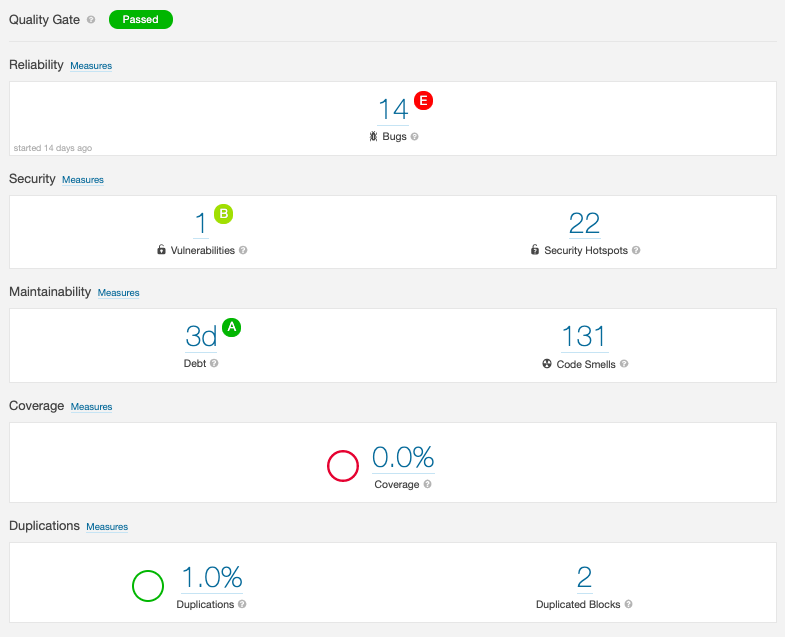
\includegraphics[scale = 0.45]{sonarEvaluation.png}

  \caption {Menu geral de avaliação do SonarQube}

  \label {fig01}

\end{figure}


\par Como se pode ver pela figura~\ref{fig01} este projeto possui alguns bugs, pelo menos 1 vulnerabilidade uma quantidade consideravel de code smells e 2 blocos duplicados.


De seguida apresenta-se um relatório detalhado dos tipos de erros e da sua gravidade:
\subsection{Bugs}
versão com bugs, sem bugs, com smells sem smells (por tipos de smells) -> descriminar o impacto dos smells
\subsubsection{Blocker Bugs:}
\begin{itemize}
\item Não usar blocos try/catch ao escrever em ficheiros.\newline
 Ficheiro: UMCarroJa.java\newline


\par Podemos visualizar nas seguintes imagens o código analisado e a solução respetiva.

\begin{figure}[H]

  \centering

  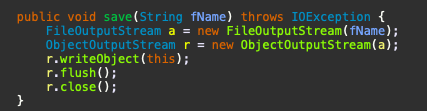
\includegraphics[scale = 0.5]{preWriteTryCatch.png}

  \caption {Código com bug}

  \label {fig02}

\end{figure}

\begin{figure}[H]

  \centering

  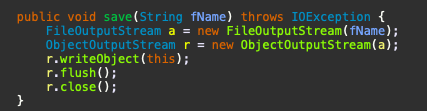
\includegraphics[scale = 0.5]{posWriteTryCatch.png}

  \caption {Código corrigido}

  \label {fig03}

\end{figure}

\item Não usar blocos try/catch ao ler de ficheiros.\newline
 Ficheiro: UMCarroJa.java\newline


\par Podemos visualizar nas seguintes imagens o código analisado e a solução respetiva.


\begin{figure}[H]

  \centering

  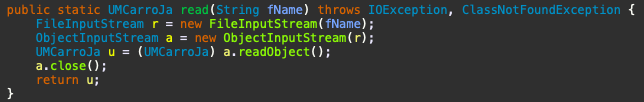
\includegraphics[scale = 0.5]{preReadTryCatch.png}

  \caption {Código com bug}

  \label {fig04}

\end{figure}

\begin{figure}[H]

  \centering

  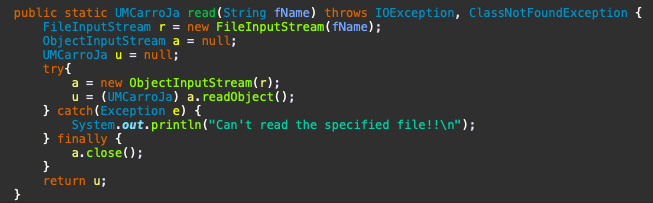
\includegraphics[scale = 0.5]{posReadTryCatch.png}

  \caption {Código corrigido}

  \label {fig05}

\end{figure}

\end{itemize}
\par Note-se que é usado no fim dos blocos \textit{try/catch} o bloco \textit{finally} para fechar o descritor de escrita/leitura. Isto serve para, caso alguma coisa corra mal na escrita em/leitura de um ficheiro, o descritor ser fechado. 

\subsubsection{Critical Bugs:}
\begin{itemize}
\item Guardar e reutilizar variáveis random.\newline
 Ficheiro: Traffic.java \newline


\par Para resolver o problema basta verificar que o random estava a ser gerado sempre que a função \textit{getTraficDelay()} era invocada. Para resolver basta gerar o random uma unica vez quando a classe for criada e usar o mesmo sempre que a função em causa for invocada.

\begin{figure}[H]

  \centering

  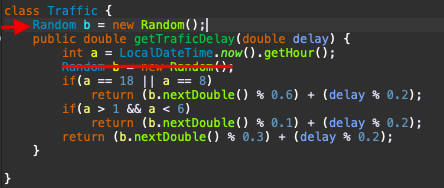
\includegraphics[scale = 0.5]{randomGeneration.png}

  \caption {Recolocação do método de geração de um número Random}

  \label {fig06}

\end{figure}
\end{itemize}

\subsubsection{Major Bugs:}
\begin{itemize}
\item Não obrigar a usar o método redifinido usando override.\newline
 Ficheiro: Car.java\newline


.................Rever...............
\par Para resolver este problema fo preciso renomear o método equals para o método isEqual, visto que usando um \textit{@Override} este método obrigaria a implementar um método de super tipo.

\begin{figure}[H]

  \centering

  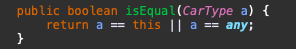
\includegraphics[scale = 0.5]{isEqualFunction.png}

  \caption {Definição da função isEqual}

  \label {fig07}

\end{figure}

\end{itemize}

\subsubsection{Minor Bugs:}
\begin{itemize}
\item Obrigar o override do equals e não o do método hashCode().\newline
 Ficheiros: Car.java, Cars.java, Cliente.java, Owner.java, Parser.java, Rental.java, Rentals.java, User.java, Users.java.\newline


\par Para corrigir este problema, basta definir um hashCode() que chame super.hashCode() como se pode ver na figura seguinte.

\begin{figure}[H]

  \centering

  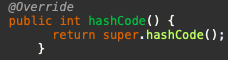
\includegraphics[scale = 0.6]{hashCode.png}

  \caption {Solução do problema de Override do método hashCode}

  \label {fig08}

\end{figure}

\end{itemize}


\subsection{Vulnerabilitys}
\begin{itemize}
\item Utilizar printStackTrace() pode revelar informação sensivel.\newline
 Ficheiro: Parser.java\newline
\end{itemize}

\subsection{CodeSmells}

\subsubsection{Blocker CodeSmells:}
\subsubsection{Critical CodeSmells:}
\begin{itemize}
\item Possuir um método complexo com cerca de de 290 linhas, é muito dificil manter e até mesmo perceber um código tão extenso.\newline
 Ficheiro: Controller.java\newline

\par Para resolver o problema cada case do switch foi dividido em 1 função de complexidade inferior de média 15 linhas. podemos ver nas duas figuras em baixo, um dos cases e a função para o qual foi passado o código correspondente.

\begin{figure}[H]

  \centering

  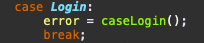
\includegraphics[scale = 0.6]{newSmallerCase.png}
  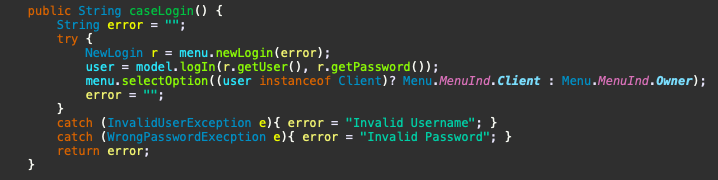
\includegraphics[scale = 0.6]{newSmallerFunction.png}

  \caption {Solução do problema complexidade extrema do método run()}

  \label {fig10}

\end{figure}
\end{itemize}

\begin{itemize}
\item Repetir várias vezes a atribuição da mesma string pode tornar o código confuso. \newline
\par Para ultrapassar essa dificuldade essa string passou a ser criada e guardade numa variável quando um objeto da classe é inicializado e essa variável é depois atribuida quando necessário. \newline
 Ficheiro: Controller.java\newline
\end{itemize}





\subsubsection{Major CodeSmells:}



\subsubsection{Minor CodeSmells:}
\begin{itemize}
\item Nomes de pacotes com letras maiúsculas.\newline
 Ficheiros: todos os packages exceto o main.java.\newline


\par Para resolver este problema basta substituir as letras maiúsculas nos nomes dos packages por minusculas, o eclipse trata de renomear o nome do package nas declarações feitas dentro dos ficheiros do próprio package.\newline
\par Em seguida temos um exemplo da correção de uma dessas ocorrencias. 
\begin{figure}[H]

  \centering

  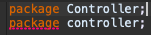
\includegraphics[scale = 0.6]{packageRename.png}

  \caption {Solução do problema de renomeação de packages}

  \label {fig09}

\end{figure}

\end{itemize}

\begin{itemize}
\item Utilização de métodos ineficientemente.\newline
 Ficheiros: Controller.java e Menu.java.\newline


\par Neste caso num if é utilizado o método size() do ArrayList e seguidamente verifica-se se o array está vazio. A solução para esta ineficiencia passa por invocar o método isEmpty() do ArrayList.\newline
\par Em seguida temos um exemplo da correção de uma dessas ocorrencias. 
\begin{figure}[H]

  \centering

  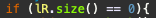
\includegraphics[scale = 0.6]{sizeForIsEmpty.png}

  \caption {Solução do problema de inefeciência no uso de funções de Coleções na classe Controller}

  \label {fig10}

\end{figure}


\par Como na classe \textit{Menu.java} foi preciso trocar a execução do if com o else, para uma melhor percepção do que foi feito, a mudança será mostrada no figura seguinte.

\begin{figure}[H]

  \centering

  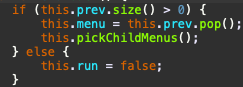
\includegraphics[scale = 0.6]{ifElseChangePre.png}
  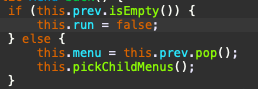
\includegraphics[scale = 0.6]{ifElseChangePos.png}

  \caption {Solução do problema de inefeciência no uso de funções de Coleções na classe Menu}

  \label {fig11}

\end{figure}

\end{itemize}

\begin{itemize}
\begin{itemize}
\item Classe sem package.\newline
 Ficheiro: main.java.\newline


\par Neste caso basta declarar o package a que a classe pertence, como se pode ver na figura seguinte.\newline 

\begin{figure}[H]

  \centering

  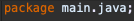
\includegraphics[scale = 0.6]{packageMainJava.png}

  \caption {Declaração do package a que a classe main.java pertence}

  \label {fig12}

\end{figure}

\end{itemize}

\begin{itemize}
\item Utilização de métodos ineficientemente.\newline
 Ficheiro: Car.java.\newline


\par Para colmatar a ineficiencia do código basta mudar a negação de uma operação de >, extremamente custosa, para uma operação de >= que tem o mesmo efeito.\newline
\par A resolução encontra-se na figura seguinte. 
\begin{figure}[H]

  \centering

  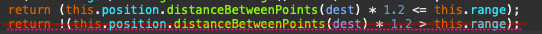
\includegraphics[scale = 0.6]{returnMinorEqual.png}

  \caption {Solução do problema de inefeciência do return}

  \label {fig13}

\end{figure}

\end{itemize}

\begin{itemize}
\item Declaração de um clone() sem \textit{@Override}.\newline
 Ficheiro: Car.java, Cars.java, Cliente.java, Owner.java e Point.java.\newline


\par Para resolver o problema basta adicionar o \textit{@Override} no método, como se pode ver na seguinte figura.\newline

\begin{figure}[H]

  \centering

  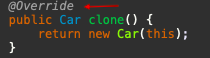
\includegraphics[scale = 0.6]{overrideCloneCar.png}


  \caption {Implementação do método clone() da classe Car}

  \label {fig14}

\end{figure}

\end{itemize}


\begin{itemize}
\item Método devolve ArrayList em vez de List, dando informação sobre a implementação do método.\newline
 Ficheiro: Cars.java, Owner.java.\newline


\par Para resolver o problema basta por o método a devolver uma interface genérica.\newline
\par Note-se que as funções que invocam estes métodos devem ser corrigidas declarando o tipo recebido com \textit{(ArrayList<Rental>)}.

\begin{figure}[H]

  \centering

  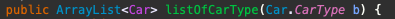
\includegraphics[scale = 0.6]{returningArrayList.png}
  
\includegraphics[scale = 0.6]{returningList.png}

  \caption {Exemplo da mudança do tipo de interface retornada por um método}

  \label {fig15}

\end{figure}

\end{itemize}

\begin{itemize}
\item Utilização desnecessária de parentesis num filter.\newline
 Ficheiro: Cars.java e UmCarroJa.java.\newline


\begin{figure}[H]

  \centering

  
\includegraphics[scale = 0.6]{filterEpre.png}
  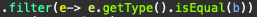
\includegraphics[scale = 0.6]{filterEpos.png}

  \caption {filter sem paretesis}

  \label {fig16}

\end{figure}

\end{itemize}


\begin{itemize}
\item Declaração de variáveis pela ordem errada, dificultando a leitura do código, estão declaradas da seguinte ordem: static final, final, private. Na figura podemos ver a ordem reescrita da forma correta. \newline
 Ficheiro: Rentals.java.\newline


\begin{figure}[H]

  \centering

  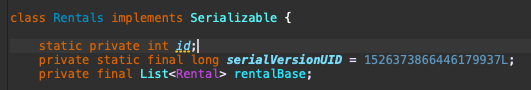
\includegraphics[scale = 0.6]{reorderDeclarations.png}

  \caption {Ordenação correta das declarações de variáveis}

  \label {fig17}

\end{figure}

\end{itemize}

\begin{itemize}
\item Declaração de um método em com a primeira letra maiúscula, o nome Original deste era \textit{RESET()}. \newline
 Ficheiro: StringBetter.java.\newline


\begin{figure}[H]

  \centering

  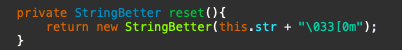
\includegraphics[scale = 0.6]{resetFunction.png}

  \caption {Declaração correta do método, usando letra minúscula no início}

  \label {fig18}

\end{figure}

\end{itemize}

\begin{itemize}
\item Declaração de um método fazendo uso de um underscore no seu nome, seguindo a expressão regular da nomeação de métodos estes não devem ter underscore.De seguida apresenta-se um exemplo de um dos métodos corrigidos. \newline
 Ficheiro: StringBetter.java.\newline


\begin{figure}[H]

  \centering

  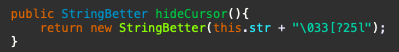
\includegraphics[scale = 0.6]{renameFunction.png}

  \caption {Declaração correta do método retirando o underscore e substituindo letra seguinte por maiúscula}

  \label {fig19}

\end{figure}

\end{itemize}

\begin{itemize}
\item Declaração de variáveis começadas por letra maiúscula. \newline
 Ficheiro: NewLogin.java.\newline

\par Apesar de não ser mostrado, no método NewLogin(), o nome e a password também foram modificado para fazer match com a renomeação demonstrada na figura.

\begin{figure}[H]

  \centering

  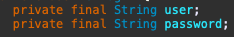
\includegraphics[scale = 0.6]{varsMaiusculas.png}

  \caption {Declaração correta das variáveis user e password}

  \label {fig19}

\end{figure}

\end{itemize}





